% \documentclass[oneside]{report}
\documentclass[oneside,final,14pt,a4paper]{extreport}
\usepackage[T2A]{fontenc}

\usepackage{microtype}

\usepackage{vmargin}
\setpapersize{A4}
\setmarginsrb{2.5cm}{2cm}{2cm}{2cm}{0pt}{10mm}{0pt}{13mm}
\usepackage{setspace}
\sloppy
\setstretch{1.5}
\usepackage{indentfirst}
\parindent=1.25cm

%%%%% ADDED TO SUPPORT TT BOLD FACES %%%%
\DeclareFontShape{OT1}{cmtt}{bx}{n}{<5><6><7><8><9><10><10.95><12><14.4><17.28><20.74><24.88>cmttb10}{}
\renewcommand{\ttdefault}{pcr}
%%%%% END %%%%%%%%%%%%%%%%%%%%%%%%%%%%%%% 
\usepackage{atbegshi,picture}
\AtBeginShipout{\AtBeginShipoutUpperLeft{%
  \put(\dimexpr\paperwidth-1cm\relax,-1.5cm){\makebox[0pt][r]{
\includegraphics[width=3cm]{figs/inno}}}%
}}


\usepackage[english]{babel}
\usepackage[backend=biber,style=ieee,autocite=inline,citestyle=authoryear,maxcitenames=1,mincitenames=1]{biblatex}
\bibliography{ref.bib}
\DefineBibliographyStrings{english}{%
  bibliography = {References},}

\usepackage{pdfpages}
\newenvironment{bottompar}{\par\vspace*{\fill}}{\clearpage}
\usepackage{amsmath,amsfonts}

\usepackage{amsthm}
\newtheorem{theorem}{Theorem}
\newtheorem{corollary}{Corollary}
\newtheorem{lemma}{Lemma}
\newtheorem{proposition}{Proposition}
\theoremstyle{definition}
\newtheorem{definition}{Definition}
\theoremstyle{remark}
\newtheorem*{remark}{Remark}
\theoremstyle{remark}
\newtheorem*{example}{Example}



\usepackage{float}
\usepackage{graphicx}
\graphicspath{{figs/}} %path to images
\usepackage{array}
\usepackage{multirow,array}
\usepackage{caption}
\usepackage{subcaption}
\usepackage{hyperref}
\usepackage{paralist}
\usepackage{listings}
\usepackage{zed-csp}
\usepackage{fancyhdr}
\usepackage{csquotes}
\usepackage{color}
\usepackage[ruled]{algorithm2e}

\usepackage{upgreek} 
\usepackage{bm}
\usepackage{hyperref}
\usepackage{setspace}
\usepackage{booktabs}
\usepackage{multirow}
\usepackage{longtable}
\usepackage[font=singlespacing, labelfont=bf]{caption}

\counterwithout{table}{chapter}
\renewcommand{\thetable}{\Roman{table}}

%Hints
\newcommand\pic[1]{(Fig. \ref{#1})} %Ref on figure
\newcommand\tab[1]{(Tab. \ref{#1})} %Ref on table


\usepackage{enumitem}
\newlist{inlinelist}{enumerate*}{1}
\setlist*[inlinelist,1]{%
  label=(\arabic*),
}

\lstdefinestyle{code_snippet} {
    commentstyle=\color{gray},
    keywordstyle=\color{blue},
    numberstyle=\tiny\color{blue},
    stringstyle=\color{green},
    basicstyle=\ttfamily\footnotesize,
    breakatwhitespace=false,         
    breaklines=true,                 
    captionpos=b,                    
    keepspaces=true,                 
    numbers=left,                    
    numbersep=5pt,                  
    tabsize=2,
    frame=single
}

\lstset{style=code_snippet}


\pagestyle{fancyplain}

% remember section title
\renewcommand{\chaptermark}[1]%
	{\markboth{\chaptername~\thechapter~--~#1}{}}

% subsection number and title
\renewcommand{\sectionmark}[1]%
	{\markright{\thesection\ #1}}

\rhead[\fancyplain{}{\bf\leftmark}]%
      {\fancyplain{}{\bf\thepage}}
\lhead[\fancyplain{}{\bf\thepage}]%
      {\fancyplain{}{\bf\rightmark}}
\cfoot{} %bfseries
\setlength{\headheight}{17pt}


\newcommand{\dedication}[1]
   {\thispagestyle{empty}
     
   \begin{flushleft}\raggedleft #1\end{flushleft}
}

\begin{document}

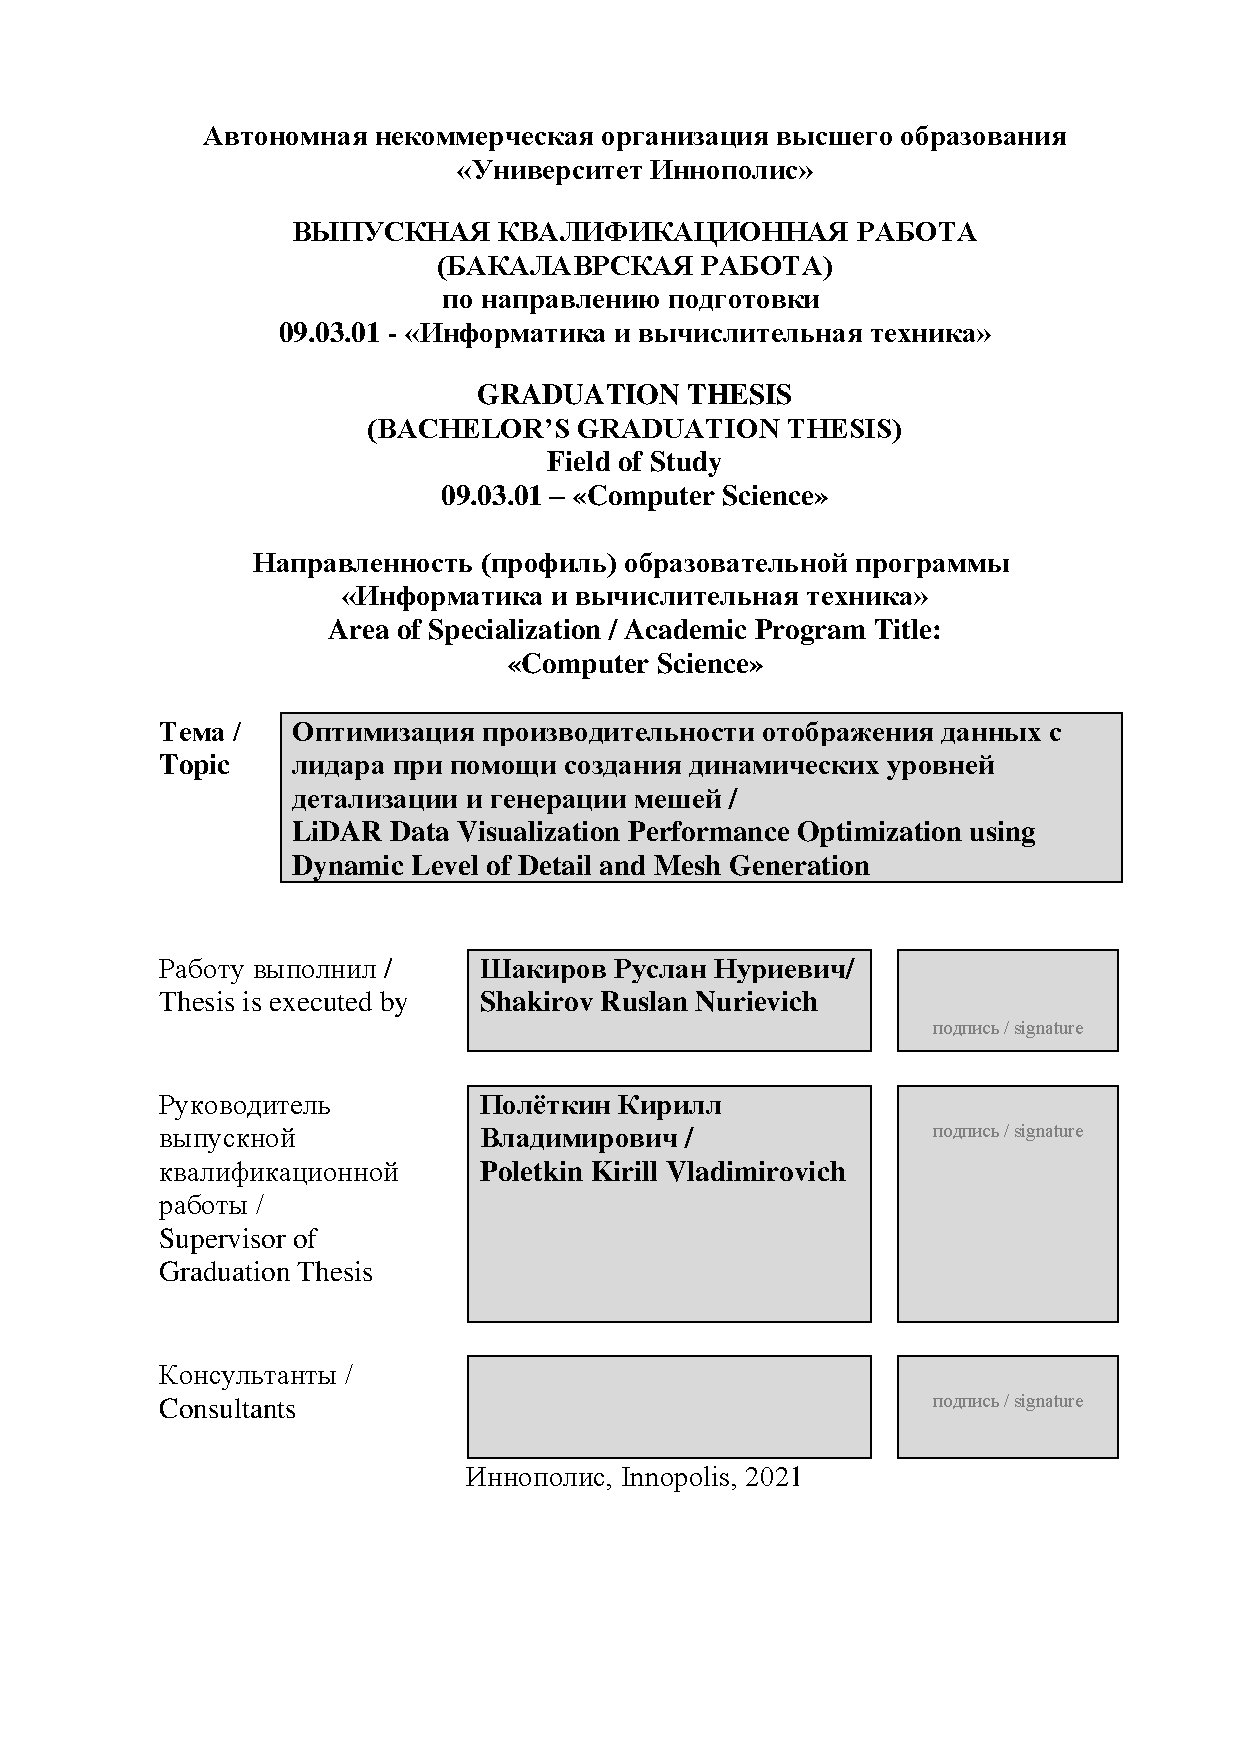
\includepdf[pages=-, offset={-\hoffset} {\voffset}]{title.pdf}
\tableofcontents
\listoftables
\listoffigures


\newpage
% \begin{abstract}

In this work, we present two methods for processing point clouds for rendering acceleration. The first method generates different levels of detail for parts of the cloud to simplify the parts of the point cloud that are barely visible. The second method reconstructs the terrain model mesh that has a smaller size and fewer vertices. As we were working on automotive simulator software, we needed to visualize terrain scans captured in the form of point clouds. Rendering unprocessed point cloud data has a significant performance impact. Thus, we decided to optimize the way we visualize point clouds. In this work, we propose two methods that we implemented as a proof of concept. The results revealed a noticeable performance improvement, so we successfully integrated these methods into the automotive simulator. Furthermore, we found ways to visualize point clouds with high performance while maintaining the visual quality on the same level as unprocessed data. Furthermore, developers who work on terrain visualizing software, vehicle simulators, and other visualization applications could consider this work for applying it in their product.

\end{abstract}

% Depend on above part
\setcounter{page}{6}
\chapter{Literature review}
\label{chap:lr}

% TODO: Make Latex references

This thesis addresses the problem slightly covered by the scholar community, and it is not easy to find related research to support this work. The absence of relevant literature highlights the research gap in the current research topic.

For this thesis, we selected six papers that fit the topic and helps us to create helpful research. There are four conference proceedings, one journal article, and one patent. These include research on generating different levels of detail for graphical objects, building terrain information based on raw scanner data, and other performance optimization techniques.

This review examined preprocessing algorithms, real-time approaches, and other auxiliary methods that we may apply in this work.

The first part of this review examines the preprocessing methods. The second part explores the real-time methods. In the end, we have a look at auxiliary methods that are not directly related to this research.


\section{Preprocessing methods}

Preprocessing the raw data plays a crucial role in optimizing the performance of further visualization. It might help us to apply more advanced methods at run time. In this section, we are going to observe the methods for point cloud data preparation.

\subsection{Estimating surface normals from noisy PCD}

\textcite{Mitra2003} proposed the method for generating terrain maps out of point cloud data (PCD). This paper also provided techniques for noise filtering. Both methods might help to improve the overall performance of our visualization software but are not fully applicable in current work because they do not involve LOD generation and operates before the run time.

\subsection{Sorting vertices}

\textcite{Evans2013} came with an algorithm for sorting the vertices before sending the point cloud data to the graphics device. Ordered data allows us to generate different levels of detail and dynamically change them continuously. However, this method involves the usage of octree maps which have high memory consumption. The question of how to efficiently store the point cloud remains open.


\section{Real-time methods}

This work assesses methods for real-time LOD generation, so it is important to examine existing solutions and their differences and drawbacks. There is no solution for the proposed problem, but different concepts might help us overcome the drawbacks.

\subsection{Real-time depth grid LODs for automotive}

\textcite{Schmid2010} introduced an algorithm for the real-time level of detail generation for depth perception data from LiDAR installed in a car. It involves simple mathematical computations, and we can potentially apply it for visualizing recorded data. Although this method operates with LiDAR-generated point clouds, the algorithm does not operate with point vertices. Instead, it uses a depth grid with dynamically changing resolution. We found the mathematical foundations introduced in this method helpful for this work.

\subsection{Generating LODs using tessellation}

In their book, \textcite{Malik2000} came with another suitable approach for real-time visualization – tessellation-based LOD generation. The main advantage of this method is that it utilizes the base functionality of modern graphics hardware – tessellation. It means that we can efficiently generate different levels of detail in run time. However, the method uses terrain data rather than raw point cloud data, but it might be possible to adapt the concepts of this algorithm to our needs.


\section{Auxiliary methods}

Some auxiliary methods cannot be directly applied to point cloud data, but we found some parts helpful for preparing and visualizing the data.

\subsection{Assessing the impact on performance for different LODs}

\textcite{Minarno2020} observed a method for generating terrain with different levels of detail (LOD) by reducing the amount of data used to generate meshes. Also, this paper assessed the impact on resource usage and overall performance for different LODs and provided the correlation data for performance/detail metrics. However, this work did not emphasize the process of LOD creation. Instead, it paid more attention to statistics collection and comparison.

\subsection{Visualizing complex meshes with different LODs}

\textcite{Callahan2005} proposed an algorithm for generating a dynamic level of detail based on sampling techniques. The authors examined four different approaches to down-sampling. This work has a significant advantage – the authors designed the algorithm to execute on graphics hardware (GPU). However, this method needs adaptation for visualizing point clouds as original implementation approaches complex mesh visualization. It is unclear whether we can apply the algorithm at run time, and this question needs further investigation.

\chapter{Methodology}
\label{chap:methodology}

\graphicspath{{figs/methodology/}}

\section{Point Cloud Data}
\label{sec:point_cloud_data}

This project aims to work with large amounts of point cloud data. It contains arrays of three-dimensional coordinates and the four-component color data. The color information does not affect performance strongly. However, the massive number of points itself introduces the heavy load on computer resources. For improving the performance of visualization software, this work proposes two methods: Generating Levels of Detail (LODs) and Creating a heightmap.


\section{Data Preprocessing}
\label{sec:data_preprocessing}

The data itself is stored in a PCAP file as captured packet stream from the lidar. It is necessary to preprocess original files before working on the point cloud. The preprocessing involves three main steps: converting the file from PCAP format to the LAS format, importing the LAS file into Unity, and splitting the point cloud data into chunks.

\subsection{Splitting into chunks}

For the proposed methods it is crucial to split the point cloud into smaller units (chunks) that are easier to process. It also helps to process the data in a parallel manner, thereby making the algorithms more scalable in terms of performance.

In terms of the given project, the chunk is a space bounded by computed borders. It has a position, and a size, which is the same for its width, height, and depth. 

\paragraph{Algorithm}
At the start, the algorithm computes the number of chunks in three dimensions using the formula \ref{eqn:n_chunks}. It uses the predefined chunk size and the boundaries of the point cloud object.

The number of chunks for an axis $\alpha$ is computed as follows:

\begin{equation}
\label{eqn:n_chunks}
N_{chunks}^\alpha = \lceil BBox_{max}^\alpha - BBox_{min}^\alpha \rceil / Size_{chunk}
\end{equation}

For that, the chunk grid will have the size of $N_{chunks}^X \times N_{chunks}^Y \times N_{chunks}^Z$.

The chunks are stored in a three-dimensional array. It means that each chunk has its corresponding index.

After that, the algorithm iterates overall points and computes the exact chunk index they correspond to, based on their global position.

The chunk index for a point with position $pos$ on an axis $\alpha$ is computed as shown on formula \ref{eqn:point_index}:

\begin{equation}
\label{eqn:point_index}
Index_{pos}^\alpha = \left \lfloor \frac{pos^{\alpha} - BBox_{min}^\alpha}{Size_{chunk}} \right \rfloor
\end{equation}

In the end, the points are stored within chunks. It is now possible to read the point cloud data in chunks.


\section{Method 1: Generating LODs}
\label{sec:generating_lods}

The level of detail defines the complexity of the model [citation here]. For this project, the level of detail adjusts the number of points shown for a particular object.
The LOD of $L$ shows $L\%$ of all points of an object. For example, a chunk with LOD 100 contains all its points while a chunk with LOD 75 has $75\%$ of its points.

\begin{figure}[h]
    \centering
    
    \begin{subfigure}{0.2\textwidth}
        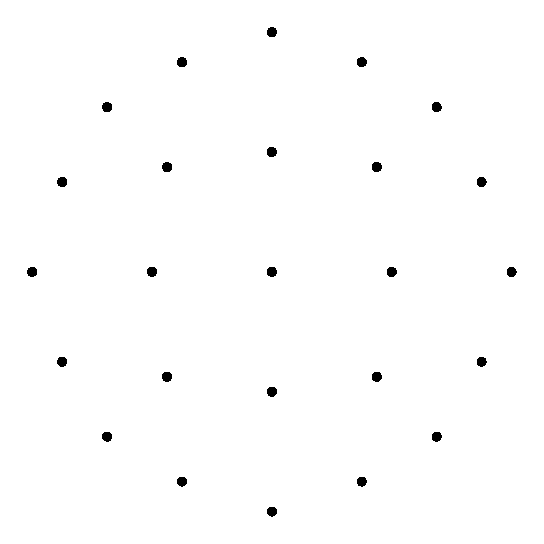
\includegraphics[width=\textwidth]{lod-cloud-25.pdf}
        \caption{$LOD = 25$}
    \end{subfigure}
    % side-by-side
    \begin{subfigure}{0.2\textwidth}
        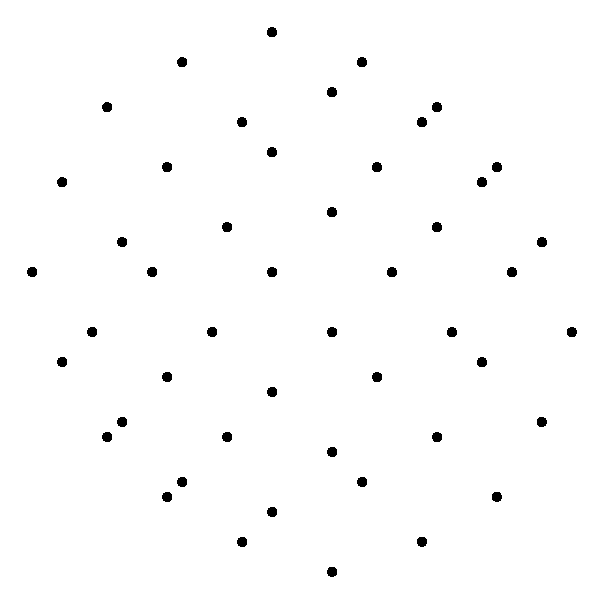
\includegraphics[width=\textwidth]{lod-cloud-50.pdf}
        \caption{$LOD = 50$}
    \end{subfigure}
    % side-by-side
    \begin{subfigure}{0.2\textwidth}
        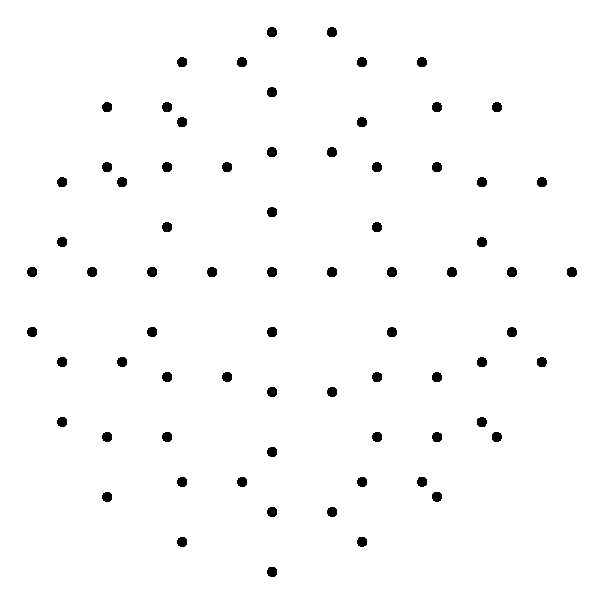
\includegraphics[width=\textwidth]{lod-cloud-75.pdf}
        \caption{$LOD = 75$}
    \end{subfigure}
    % side-by-side
    \begin{subfigure}{0.2\textwidth}
        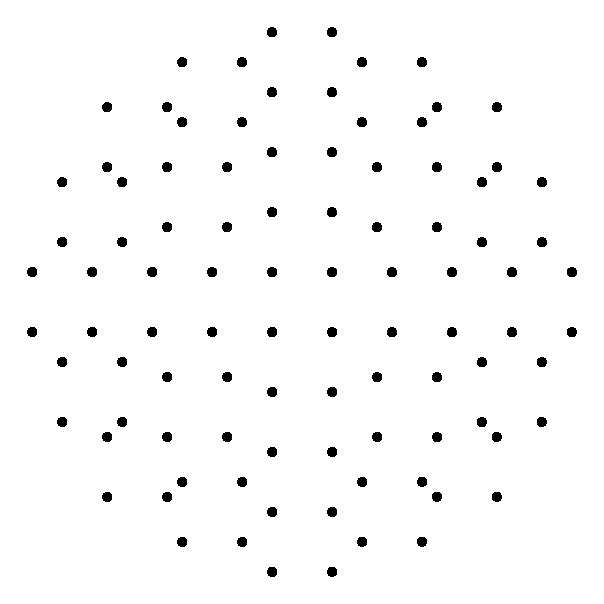
\includegraphics[width=\textwidth]{lod-cloud-100.pdf}
        \caption{$LOD = 100$}
    \end{subfigure}
    
    \caption{Different LODs of a point cloud.}
    \label{fig:cloud_lods}
\end{figure}

The approach is to generate different levels of detail for each chunk, so it will be possible to show fewer points for chunks that are far enough not to notice the low-detailed chunk.

\subsection{Reducing the number of points}

When loading the data with a specific LOD, the algorithm takes each $stride^{th}$ element from the set of all chunk points. Stride is calculated using the \autoref{eqn:lod_stride}.

\begin{equation}
\label{eqn:lod_stride}
stride(LOD) = \frac{100}{LOD}
\end{equation}

\begin{figure}[htb]
    \centering
    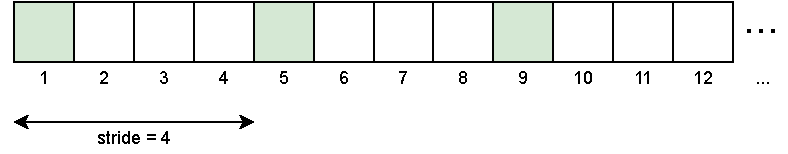
\includegraphics[width=0.8\textwidth]{lod-stride.pdf}
    \caption{Example of stride with $LOD = 25$. In that case $stride(25)=4$.}
    \label{fig:stride}
\end{figure}

\begin{algorithm}
    \caption{Picking points with stride.}
    
    int i $\gets$ 0\;
    Point[$\;$] newPoints $\gets$ [$\;$]\;
    \For{p in points}{
        \If{i \% stride == 0}{
            newPoints.add(p)\;
        }
    }
\end{algorithm}

Different levels of detail are pregenerated for each chunk. The algorithm generates distinct assets \footnote{Asset is an item that can be used within an application (3D model, picture, audio, code, etc.).} for each requested LOD.

When visualization is in progress, the LOD for each chunk is selected based on the distance between the viewer and the chunk. A user predefines the distances and corresponding LODs. The distance between two objects can be computed using the Pythagorean theorem (\autoref{eqn:pythagorean_3d}) as the coordinates are available for all objects.

\begin{equation}
\label{eqn:pythagorean_3d}
distance(p_1, p_2) = \sqrt{(p_1^x-p_2^x)^2 + (p_1^y-p_2^y)^2 + (p_1^z-p_2^x)^2}
\end{equation}

\subsection{Time complexity}

This algorithm traverses all chunk points once, so the complexity can be evaluated to $\mathcal{O}(n)$ (where $n$ is the number of points in a chunk), assuming that copying a point has constant complexity.


\section{Method 2: Creating a Mesh}
\label{sec:creating_mesh}

Mesh is a data structure that contains vertices, texture data, normals, and other details [citation here]. Later, the engine  combines the mesh data and draws it on the scene.

Mesh creation consists of several stages:

\begin{enumerate}
    \item Map the point cloud into grid.
    \item Generate triangles.
    \item Fill the mesh.
\end{enumerate}


\subsection{Vertex grid}

Meshes consist of vertices. We first create a set of vertices that later will form the mesh.

First, the algorithm generates a flat grid of vertices. It is a square-bounded grid-aligned region that has a specified side length. It has $length \times length$ dimensions. Each point at this plane has a height value initially set to zero.

\begin{figure}[ht]
    \centering
    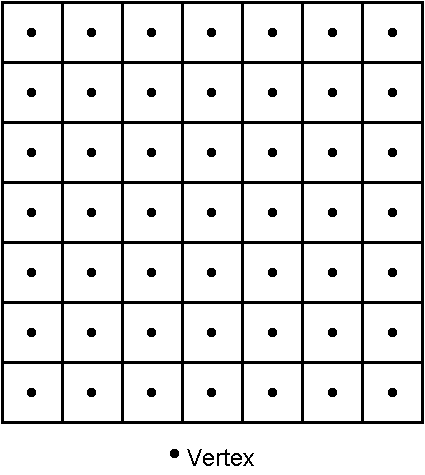
\includegraphics[width=0.3\textwidth]{vertex-grid.pdf}
    \caption{Vertex grid}
    \label{fig:vertex_grid}
\end{figure}


\subsection{Mapping the point cloud into grid}

\subsubsection{Occurrence map}

To determine where the mesh triangles should appear, the algorithm fills the occurrence map. The \textbf{occurrence map} tracks the appearance of points within the specified grid cells. It has the same size as the vertex grid. All map values are initially set to false. It means that no points have been noticed here yet.

The algorithm maps each point within a chunk to a specific occurrence map cell.

\begin{figure}[ht]
    \centering
    
    \begin{subfigure}[t]{0.3\textwidth}
        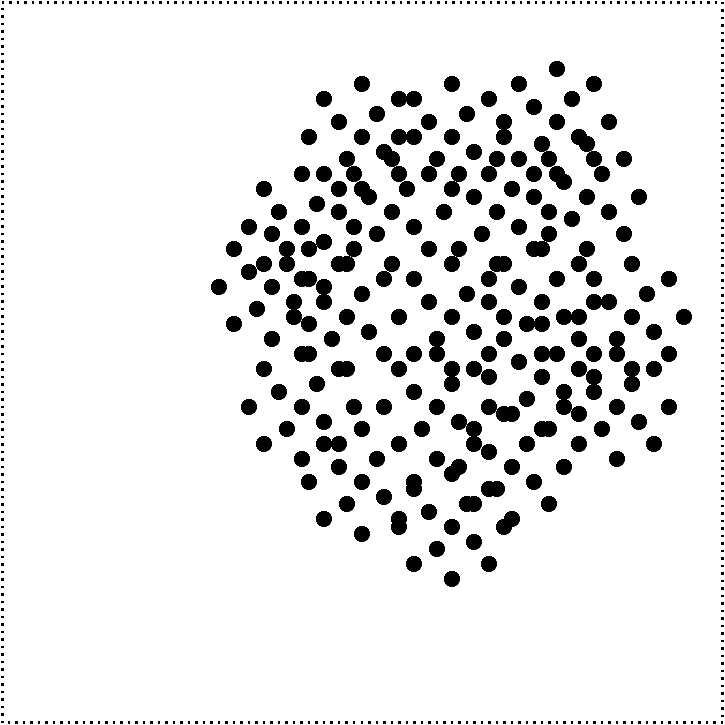
\includegraphics[width=\textwidth]{point-cloud-plot.pdf}
        \caption{Example of point cloud data in two dimensions.}
    \end{subfigure}
    % side-to-side
    \begin{subfigure}[t]{0.3\textwidth}
        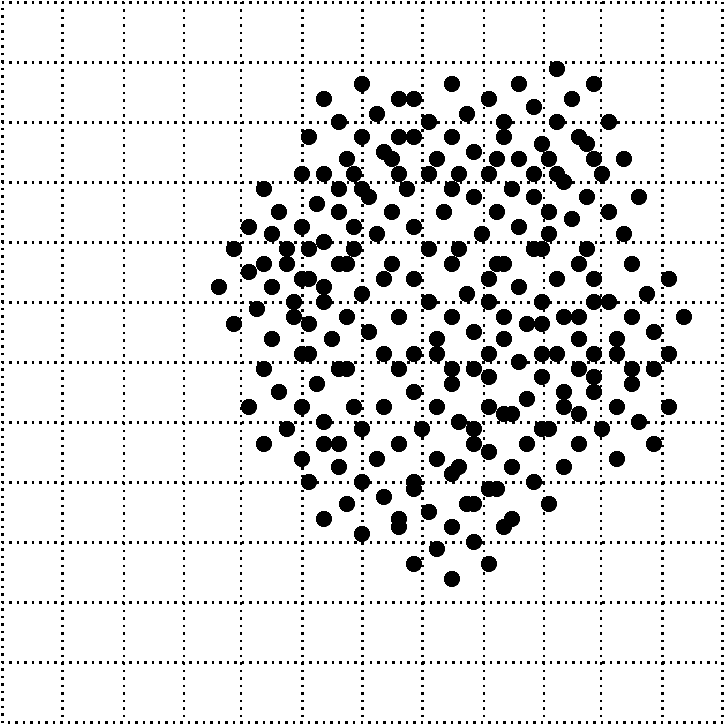
\includegraphics[width=\textwidth]{occurrence-grid.pdf}
        \caption{Occurrence grid.}
    \end{subfigure}
    
    \begin{subfigure}[t]{0.4\textwidth}
        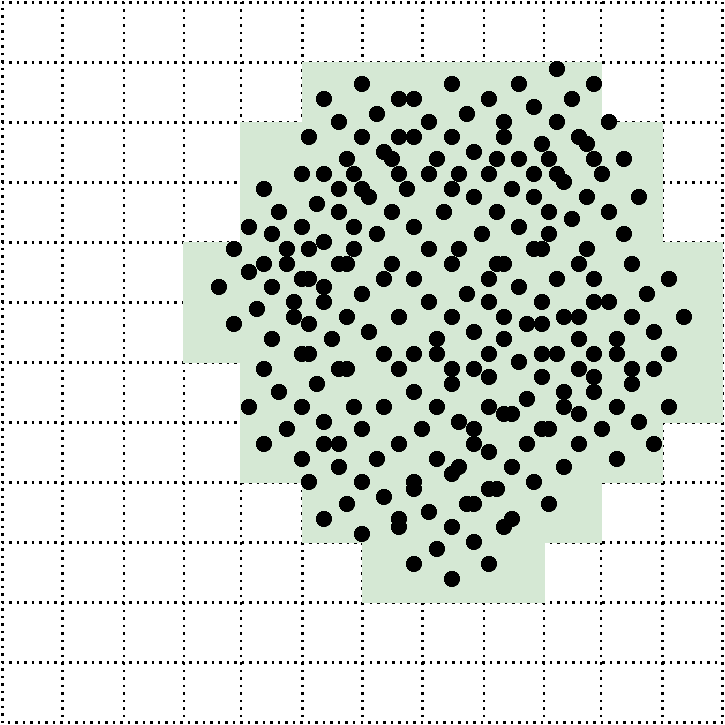
\includegraphics[width=\textwidth]{occurrence-map-applied.pdf}
        \caption{Applied occurrence map.}
    \end{subfigure}
    
    \caption{Applying occurrence map.}
    \label{fig:occurrence_map}
\end{figure}

The occurrence map represents a strictly aligned version of the point cloud viewed from above.


\subsubsection{Calculating cell indices}

To work with grid, the algorithm should calculate a cell index for each point.

To calculate an index, it should do the following:
\begin{enumerate}
    \item Calculate the local coordinate within chunk.
    \item Divide the local coordinate by cell size.
    \item Truncate the result down.
\end{enumerate}

See the formula \ref{eqn:cell_coordinate}.

\begin{equation}
\label{eqn:cell_coordinate}
Cell coordinate(p) = \left \lfloor \frac{Pos(p) - chunk origin}{cell size} \right \rfloor
\end{equation}


\subsection{Traversing points and emitting new vertices}

After initializing the vertex grid and occurrence map, the algorithm starts processing the point cloud itself.

For each point in a point cloud, the algorithm  calculates its grid cell index and fills the corresponding cell in the vertex grid and occurrence map.

At the vertex grid, the algorithm compares the height value stored in the cell and the height of the point (its Y coordinate). If the value stored in the grid is less than the point height, the algorithm writes the point height to the grid cell.

At the occurrence map, the algorithm tracks the occurrence of the points in the grid cells. If a point belongs to the cell, that cell is marked as visited.


\begin{algorithm}
    \caption{Filling the vertex grid and occurrence map.}

    \For{point \textup{p} in \textup{points}}{
        x, y, z $\gets CellCoords(p.Position)$\;
        
        \If{vertices[x,z].y < y}{
            vertices[x,z].y = y\;
        }
        
        occurrenceMap[x, z] $\gets$ \textbf{true}\;
    }
\end{algorithm}


\subsection{Generating triangles}

After finishing building the vertex grid, it is necessary to combine vertices into triangles that are going to form the mesh. To achieve this, the algorithm uses the vertex grid and the occurrence map from the previous step.

The algorithm traverses the vertex grid. The main goal is to connect three adjacent points in the grid into a triangle.

The vertex grid is represented as a two-dimensional array. On each iteration, the algorithm checks each possible triangle appearance. If a triangle exists, its vertices are recorded.

To check whether it is possible to create a triangle, the algorithm checks two adjacent points on the occurrence map. At the point $(X, Y)$, it checks whether $\left \langle (X, Y), (X+1, Y) (X, Y+1) \right \rangle$ (\autoref{fig:triangle_generation:upper}) and $\left \langle (X+1, Y), (X, Y+1), (X+1, Y+1) \right \rangle$ (\autoref{fig:triangle_generation:lower}) appear on the occurrence map. If they do, the corresponding triangles are recorded.

\begin{figure}[ht]
    \centering
    
    \begin{subfigure}{0.3\textwidth}
        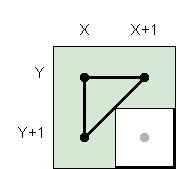
\includegraphics[width=\textwidth]{triangles-upper.pdf}
        \caption{Upper triangle.}
        \label{fig:triangle_generation:upper}
    \end{subfigure}
    % side-by-side
    \begin{subfigure}{0.3\textwidth}
        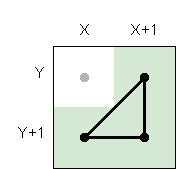
\includegraphics[width=\textwidth]{triangles-lower.pdf}
        \caption{Lower triangle.}
        \label{fig:triangle_generation:lower}
    \end{subfigure}
    % side-by-side
    \begin{subfigure}{0.3\textwidth}
        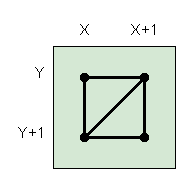
\includegraphics[width=\textwidth]{triangles-full.pdf}
        \caption{Both triangles.}
    \end{subfigure}
    
    \caption{Triangle creation. Green cells show that the cell appears on occurrence map as visited.}
    \label{fig:triangle_generation}
\end{figure}

\begin{algorithm}
    \caption{Generating triangles using occurrence map.}

    \For{\textup{x} in 1..\textup{width}}{
        \For{\textup{y} in 1..\textup{width}}{
            \If{occuranceMap[x, y] and occuranceMap[x+1, y] and occuranceMap[x, y+1]}{
                recordTriangle(x, y, x+1, y, x, y+1)\;
            }
            \If{occuranceMap[x+1, y] and occuranceMap[x, y+1] and occuranceMap[x+1, y+1]}{
                recordTriangle(x+1, y, x, y+1, x+1, y+1)\;
            }
        }
    }
\end{algorithm}

Collected sets of vertices and triangles now form the mesh. Later, it is possible to apply some refinements to it, like texture, normals, or material data.

\subsection{Time complexity}

This algorithm has two loops that are executed one after another.

The first loop traverses over all chunk points – thus, its complexity can be evaluated to $\mathcal{O}(n_1)$ (where $n_1$ is the number of points in a chunk), assuming that condition evaluation, math operations, and memory access have constant complexity.

The second loop traverses over the vertex grid, which has $length \times length$ cells. It means that its complexity can be evaluated as $\mathcal{O}(n_2)$ (where $n_2$ is the number of cells in a grid), assuming that other operations have constant complexity.

$$\mathcal{O}(n_1) + \mathcal{O}(n_2) = \mathcal{O}(n)$$


\chapter{Implementation}
\label{chap:implementation}

\graphicspath{{figs/implementation/}}

This chapter introduces the implementation details of the proposed methods. The methods are described in the Methodology chapter. First, this chapter introduces the development platform and programming tools. Then it describes the peculiarities of methods implementation on the chosen platform.

\section{Development Environment}

The Innopolis Simulator project introduced several development and business constraints. The main development constraint was the programming environment: it was required to develop the application using the Unity Platform, as the larger project already uses Unity.

\subsection{Unity Platform}

Unity Platform is a platform for creating and running 3D content [citation here].  We use it for developing the application that visualizes the scanned locations on client devices.

There are two main reasons for using an existing graphics engine:

\begin{itemize}
    \item \textit{Platform-agnostic development.} Unity claims to support a wide range of devices and platforms, including desktop and mobile devices. This aspect is important as the primary project targets mobile devices for on-the-road usage [citation here].
    
    \item \textit{Lower development costs.} Unity provides the functionality for visualization and scripting, which would require deep research or a team of highly skilled specialists to implement that functionality on our own.
\end{itemize}

Unity engine uses .NET runtime and C\# programming language for scripting API [citation here].

For implementing the point cloud visualization module, we use Unity 2020.2.


\section{Data Preprocessing}

Vehicle hardware records the lidar data in PCAP format. PCAP is an open network traffic capturing system that uses its own “.pcap” file format [citation here]. The lidar controller software receives the data in network packets and captures the incoming stream into a PCAP file. Lidar controller uses a specific VLP-16 PCAP structure that stores the lidar laser firing responses, firing time, and capturing coordinates [citation here].

\subsection{Converting to LAS format}

As mentioned above, PCAP file contains the recorded packet stream from the lidar at the time of capturing an area. It means that the data are stored as individual captures from various perspectives and at different times.

This step collects the data stream into the single point cloud, which represents the whole captured area. The resulting point cloud is stored in LAS format.

LAS is an open file format for storing 3D point cloud data developed by the American Society for Photogrammetry and Remote Sensing [citation here]. Unlike PCAP, the LAS format stores the points of the cloud as integer number triplets.

We use the VeloView software for converting the PCAP captured stream into LAS files.

\subsection{Importing LAS files into Unity}

As this project uses the Unity engine as a base, it is essential to have the ability to read LAS files within its programming environment. 

We use the LASZip.net library for reading LAS files in the C\# environment.

We created the scripted importer [citation here] to instruct Unity about LAS file loading, thus, further importing routines can be done automatically by Unity both in the editor and run time.


\section{Method 1: Generating LODs}

This method is described in detail in \autoref{chap:methodology} \autoref{sec:generating_lods}. The method implementation includes point cloud loading, generating different levels of detail, and storing the generated LODs in the asset database for a quick retrieval at run time.

\subsection{Storing different LODs in an asset database}

Unity engine supports storing and loading resources using the asset system [citation here]. It helps developers to distribute application resources in a format that is natively supported by the Unity engine.

In Unity, each LOD should have its corresponding game object [citation here]. To systematically store generated point clouds with different LODs, we used the asset database API that helps to organize the stored resource library.

In a single point cloud object, the system creates a different asset for each chunk and each level of chunk detail. Thus, the total number of assets created is $N_{assets}=N_{chunks}\times N_{LODs}$.

The project utilizes the AssetDatabase API [citation here], provided by Unity. First, the algorithm creates a folder for storing the database. Next, as the chunk is generated with requested LODs, the corresponding assets are created.

\begin{lstlisting}[language={[Sharp]C}, caption=Asset database API usage example.]
AssetDatabase.CreateFolder(directorypath, name);
AssetDatabase.CreateAsset(data, filename);
\end{lstlisting}

\subsection{Applying LODs}

Unity requires each LOD to be a separate game object that corresponds to a parent game object. From the other perspective, the main game object has several supplementary game objects that correspond to different levels of detail. These LOD game objects are managed by the LOD Group component [citation here]. Each chunk has its own LOD group that manages chunk detail levels based on the distance to the viewer.

For the major project, we proposed the following LOD distances and levels:

\begin{table}[h]
    \centering
    \begin{tabular}{l|l}
    Distance   (abstract engine units) & LOD (stride) \\ \hline
    \textless 100 & 1 \\
    100 to 200 & 8 \\
    200 to 300 & 24 \\
    \textgreater 300 & Not rendered
    \end{tabular}
    
    \caption{LOD distances and their corresponding levels.}
\end{table}

The shown settings helped us efficiently utilize the computational resources and significantly improve the performance. The detailed performance comparison and results are shown in the Results chapter.


\section{Method 2: Creating a Mesh}

This method is described in detail in \autoref{chap:methodology} \autoref{sec:creating_mesh}. The method implementation includes creating the Unity mesh structure that the engine will render at the run time.

\subsection{Initializing the vertex grid}

Vertex grid is a grid-aligned set of vertices that will later form the mesh. We initialized the vertex grid as follows:

\lstinputlisting[language={[Sharp]C}, caption=Vertex grid initialization.]{code/vertex-grid-init.cs}

Note that the second coordinate is Z, as Unity treats Y-axis as up facing. We initialized the grid as a one-dimensional array as it will be easier to iterate over vertices later.

The next step is to fill the vertex grid and the occurrence map. It is done by iterating over the array of points.

\lstinputlisting[language={[Sharp]C}, caption=Filling vertex grid.]{code/fill-vertex-grid.cs}

The system creates a list of triangles. It will contain the vertex indices that will form triangles. Next, the algorithm iterates over the occurrence map and records the triangles into the list.

\lstinputlisting[language={[Sharp]C}, caption=Generating triangles.]{code/generate-triangles.cs}

After the triangle list has been filled, we create the mesh object. The Mesh type represents a mesh in the Unity engine [citation here]. It requires triangles and vertices. Optionally, some enhancements can be added like texture, material, or shaders.

\lstinputlisting[language={[Sharp]C}, caption=Mesh creation example.]{code/create-mesh.cs}

\chapter{Results and Discussion}
\label{chap:results}

\graphicspath{{figs/results/}}

This chapter provides the performance metrics and resulting visuals of the described methods. \autoref{chap:methodology} describes these methods on a conceptual level, and \autoref{chap:implementation} unveils the implementation details.

First, this chapter describes the measuring methodology and testing environment. Then, it shows the collected results for this application without point cloud rendering acceleration and with acceleration methods applied.


\section{Measuring methodology}

\subsection{Testing environment}

We collected the results from the application running on a computer with the following technical specifications:

\begin{itemize}
    \item CPU: AMD Ryzen 7 3750H @ 2.3GHz, 4 cores (8 threads)
    \item GPU: NVIDIA GeForce GTX 1650
    \item RAM: 16 GiB DDR4
\end{itemize}

We used the Unity Editor 2020.2.2f1 to run the developed algorithms.

\subsection{Metrics}

To evaluate the result, we proposed the following metrics:

\begin{itemize}
    \item Framerate (frames per second, FPS) – this metric helps assess the algorithm's performance.
    \item Memory consumption (mebibytes, MiB) – this metric helps assess the algorithm's resource consumption.
    \item Visual quality (absence of defects, amount of detail saved) – this metric is subjective.
\end{itemize}

\subsection{Testing scenario}

It is crucial to provide the generalized testing scenario to make the testing unbiased. In terms of this work, we tested the single component of the larger software project. The \autoref{chap:introduction} gives a brief description of the major project.

The testing scenario steps are the following:

\begin{enumerate}
    \item Select the algorithm and set the parameters.
    \item Import or re-import\footnote{The asset should be reimported in case it was imported earlier with different parameters.} LAS file with the test point cloud.
    \item Add the imported point cloud to the scene.
    \item Run the scene.
    \item Collect the metrics: the framerate in the Unity Editor, the memory usage in the operating system task manager or another resource monitor, and the rendered scene on the editor screen.
\end{enumerate}


\section{Collected results}

To minimize the environmental impact on application performance results, we made ten measurements for each testing scenario. We collected the following data by averaging ten measures during the testing.


\subsection{Generating LODs}

\subsubsection{Urban environment}

In this scenario, we measured the performance of the LOD generation algorithm on the urban scene that was captured from the part of Bangkok, Thailand [citation here].

\begin{table}[h]
    \centering
    \begin{tabular}{l|l|l|l}
    LODs & FPS & Memory (GiB) & Visual quality (relative) \\ \hline
    800, 1600, 3200 & 25.1 & 3.2 & High \\
    400, 800, 1600 & 49.5 & 3.2 & Medium \\
    200, 800, 1600 & 65.3 & 3.2 & Low
    \end{tabular}
    
    \caption{Results for LOD generation algorithm on urban environment.}
    \label{tab:results:lod-urban}
\end{table}

\begin{figure}[htb]
    \centering
    
    \begin{subfigure}{0.45\textwidth}
        \centering
        \includegraphics[width=\textwidth]{lod-urban-800.jpg}
        \caption{LOD 800-1600-3200}
        \label{fig:results:lod-urban-800}
    \end{subfigure}
    %
    \begin{subfigure}{0.45\textwidth}
        \centering
        \includegraphics[width=\textwidth]{lod-urban-400.jpg}
        \caption{LOD 400-800-1600}
        \label{fig:results:lod-urban-400}
    \end{subfigure}
    
    \begin{subfigure}{0.45\textwidth}
        \centering
        \includegraphics[width=\textwidth]{lod-urban-200.jpg}
        \caption{LOD 200-800-1600}
        \label{fig:results:lod-urban-200}
    \end{subfigure}
    
    \caption{Urban scene rendered with LODs.}
\end{figure}

On the \autoref{fig:results:lod-urban-800} the picture quality is acceptable. This setting saves most of the detail and delivers a high render distance without significant quality loss. However, it is hard to examine the scene in the close distance as the emptiness between points becomes noticeable.

Unlike the previous one, on the \autoref{fig:results:lod-urban-400} this setting delivers a lower render distance, and the algorithm renders far chunks with lower quality.

On the \autoref{fig:results:lod-urban-800} the setting provides the lowest quality for the far chunks.


\subsubsection{Landscape environment}

In this scenario, we measured the performance of the LOD generation algorithm in the countryside scene that was captured nearby the Innopolis, Tatarstan, Russian Federation.

\begin{table}[htb]
    \centering
    \begin{tabular}{l|l|l|l}
    LODs & FPS & Memory (GiB) & Visual quality (relative) \\ \hline
    300, 600,   1200 & 17.0 & 2.4 & High \\
    200, 400, 800 & 21.6 & 2.4 & Meduim \\
    100, 200, 400 & 42.2 & 2.4 & Low
    \end{tabular}
    
    \caption{Results for LOD generation algorithm on landscape environment.}
    \label{tab:results:lod-landscape}
\end{table}

\begin{figure}[h]
    \centering
    
    \begin{subfigure}{0.45\textwidth}
        \centering
        \includegraphics[width=\textwidth]{lod-landscape-300.jpg}
        \caption{LOD 300-600-1200}
        \label{fig:results:lod-landscape-300}
    \end{subfigure}
    %
    \begin{subfigure}{0.45\textwidth}
        \centering
        \includegraphics[width=\textwidth]{lod-landscape-200.jpg}
        \caption{LOD 200-400-800}
        \label{fig:results:lod-landscape-200}
    \end{subfigure}
    
    \begin{subfigure}{0.45\textwidth}
        \centering
        \includegraphics[width=\textwidth]{lod-landscape-100.jpg}
        \caption{LOD 100-200-400}
        \label{fig:results:lod-landscape-100}
    \end{subfigure}
    
    \caption{Landscape scene rendered with LODs.}
\end{figure}

On the \autoref{fig:results:lod-landscape-300} the picture quality is acceptable. However, it is hard to examine the scene in the close distance as the emptiness between points becomes noticeable.

On the \autoref{fig:results:lod-landscape-200} the picture quality is acceptable. However, as fewer points are rendered, a grain appears on the model.

On the \autoref{fig:results:lod-landscape-100} the picture quality is not acceptable. Due to the low number of rendered points, a noticeable grain appeared on the model.


\subsection{Mesh generation}

\subsubsection{Urban environment}

In this scenario, we measured the performance of the mesh creation algorithm on the urban scene that was captured from the part of Bangkok, Thailand [citation here].

\begin{table}[htb]
    \centering
    \begin{tabular}{l|l|l|l}
    Chunk resolution & FPS & Memory (MiB) & Visual quality (relative) \\ \hline
    256 & 71.4 & 551.9 & High \\
    128 & 130.4 & 498.6 & Meduim \\
    64 & 182.9 & 446.0 & Low
    \end{tabular}
    
    \caption{Results for Mesh generation algorithm on urban environment.}
    \label{tab:results:mesh-urban}
\end{table}

\begin{figure}[h]
    \centering
    
    \begin{subfigure}{0.45\textwidth}
        \centering
        \includegraphics[width=\textwidth]{mesh-urban-256.jpg}
        \caption{Mesh w. chunk resolution 256}
        \label{fig:results:mesh-urban-256}
    \end{subfigure}
    %
    \begin{subfigure}{0.45\textwidth}
        \centering
        \includegraphics[width=\textwidth]{mesh-urban-128.jpg}
        \caption{Mesh w. chunk resolution 128}
        \label{fig:results:mesh-urban-128}
    \end{subfigure}
    
    \begin{subfigure}{0.45\textwidth}
        \centering
        \includegraphics[width=\textwidth]{mesh-urban-64.jpg}
        \caption{Mesh w. chunk resolution 64}
        \label{fig:results:mesh-urban-64}
    \end{subfigure}
    
    \caption{Urban scene rendered with generated mesh.}
\end{figure}

On the \autoref{fig:results:mesh-urban-256} the setting saves the most of detail on the model.

On the \autoref{fig:results:mesh-urban-128} the setting shows less detail than the previous one, but the image has less noise than in the previous setting.

On the \autoref{fig:results:mesh-urban-64} the setting drops most of the detail, and the chunk borders become noticeable.


\subsubsection{Landscape environment}

In this scenario, we measured the performance of the mesh generation algorithm in the countryside scene that was captured nearby the Innopolis, Tatarstan, Russian Federation.

\begin{table}[htb]
    \centering
    \begin{tabular}{l|l|l|l}
    Chunk resolution & FPS & Memory (MiB) & Visual quality (relative) \\ \hline
    256 & 148.8 & 453.2 & High \\
    128 & 203.6 & 425.2 & Meduim \\
    64 & 219.3 & 379.7 & Low
    \end{tabular}
    
    \caption{Results for Mesh generation algorithm on urban environment.}
    \label{tab:results:mesh-landscape}
\end{table}

\begin{figure}[h]
    \centering
    
    \begin{subfigure}{0.45\textwidth}
        \centering
        \includegraphics[width=\textwidth]{mesh-landscape-256.jpg}
        \caption{Mesh w. chunk resolution 256}
        \label{fig:results:mesh-landscape-256}
    \end{subfigure}
    %
    \begin{subfigure}{0.45\textwidth}
        \centering
        \includegraphics[width=\textwidth]{mesh-landscape-128.jpg}
        \caption{Mesh w. chunk resolution 128}
        \label{fig:results:mesh-landscape-128}
    \end{subfigure}
    
    \begin{subfigure}{0.45\textwidth}
        \centering
        \includegraphics[width=\textwidth]{mesh-landscape-64.jpg}
        \caption{Mesh w. chunk resolution 64}
        \label{fig:results:mesh-landscape-64}
    \end{subfigure}
    
    \caption{Landscape scene rendered with generated mesh.}
\end{figure}

As the scene does not contain much detail, the picture quality is equally good on all samples. However, as the chunk size decreases, the chunk borders become thicker and more noticeable and occur more often.

All rendered visuals are available in a bigger size in \autoref{appex:rendered-scenes}.

\section{Evaluation}

\subsection{Framerate}

The \autoref{fig:results:graph-fps} summarizes the results on framerate.

\begin{figure}[h]
    \centering
    
    \begin{subfigure}{0.3\textwidth}
        \centering
        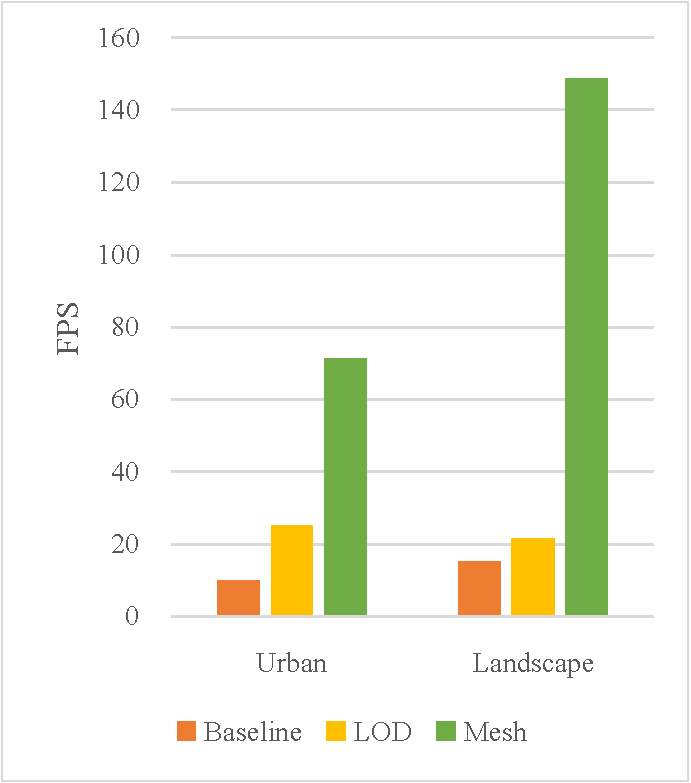
\includegraphics[width=\textwidth]{graph-fps-high.pdf}
        \caption{High quality}
    \end{subfigure}
    %
    \begin{subfigure}{0.3\textwidth}
        \centering
        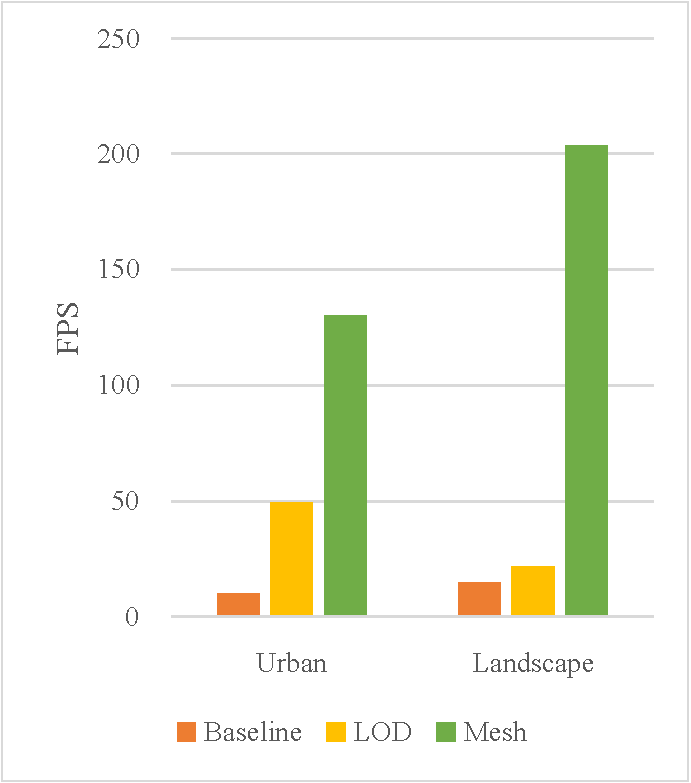
\includegraphics[width=\textwidth]{graph-fps-med.pdf}
        \caption{Medium quality}
    \end{subfigure}
    %
    \begin{subfigure}{0.3\textwidth}
        \centering
        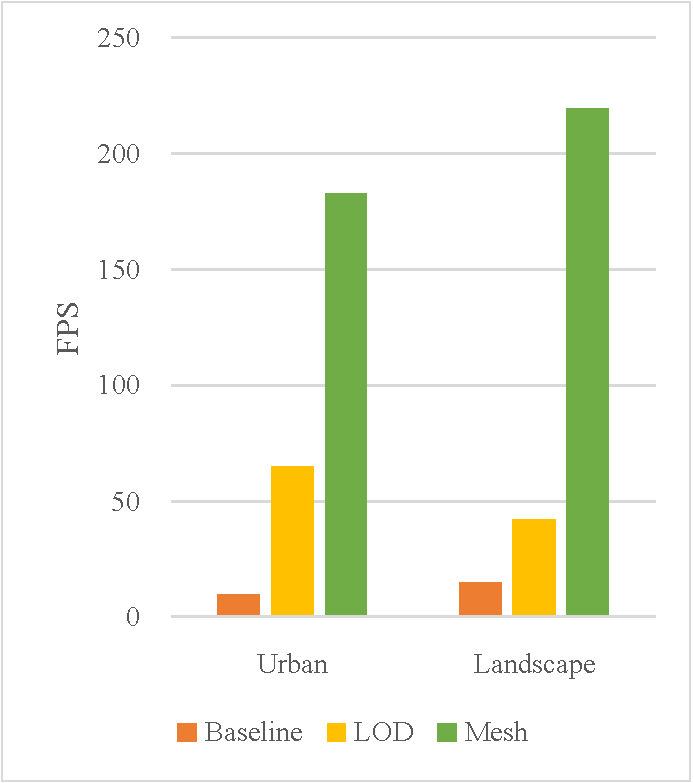
\includegraphics[width=\textwidth]{graph-fps-low.pdf}
        \caption{Low quality}
    \end{subfigure}
    
    \caption{Framerate measured on different quality settings.}
    \label{fig:results:graph-fps}
\end{figure}

The results show that the Mesh generation method demonstrates significant performance improvement over baseline and LOD generation methods.

The LOD generation method shows 2.5x to 6.5x performance improvement compared to baseline on urban scene and 1.1x to 2.8x performance improvement on landscape scene.

The Mesh generation method shows 7.1x to 18.2x performance improvement compared to baseline on urban scene and 9.9x to 14.6x performance improvement on landscape scene.

\subsection{Memory usage}

The \autoref{fig:results:graph-mem} summarizes the results on memory usage.

\begin{figure}[h]
    \centering
    
    \begin{subfigure}{0.3\textwidth}
        \centering
        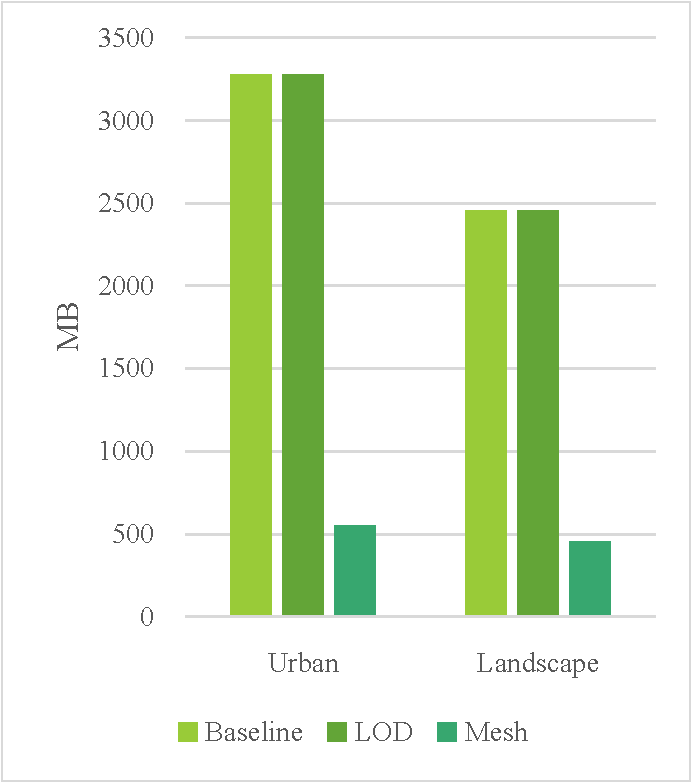
\includegraphics[width=\textwidth]{graph-mem-high.pdf}
        \caption{High quality}
    \end{subfigure}
    %
    \begin{subfigure}{0.3\textwidth}
        \centering
        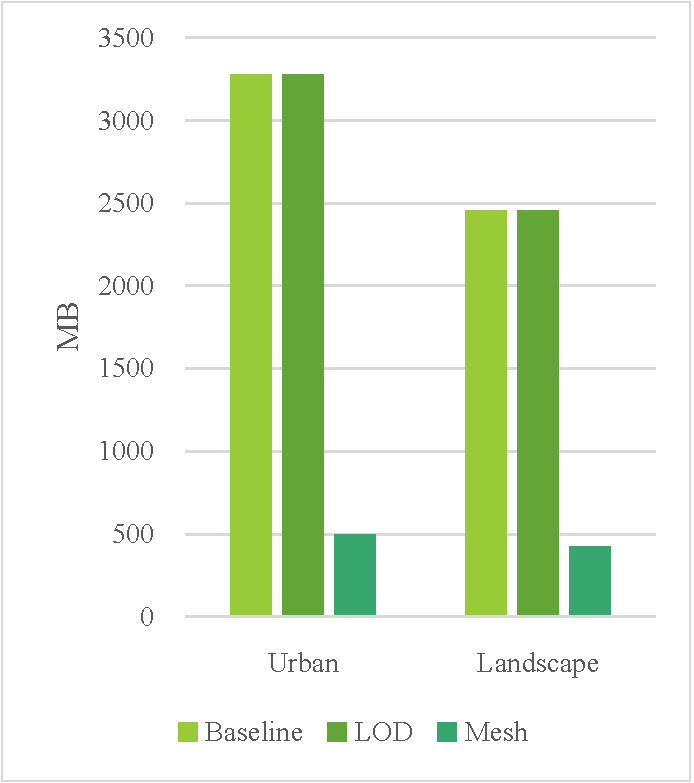
\includegraphics[width=\textwidth]{graph-mem-med.pdf}
        \caption{Medium quality}
    \end{subfigure}
    %
    \begin{subfigure}{0.3\textwidth}
        \centering
        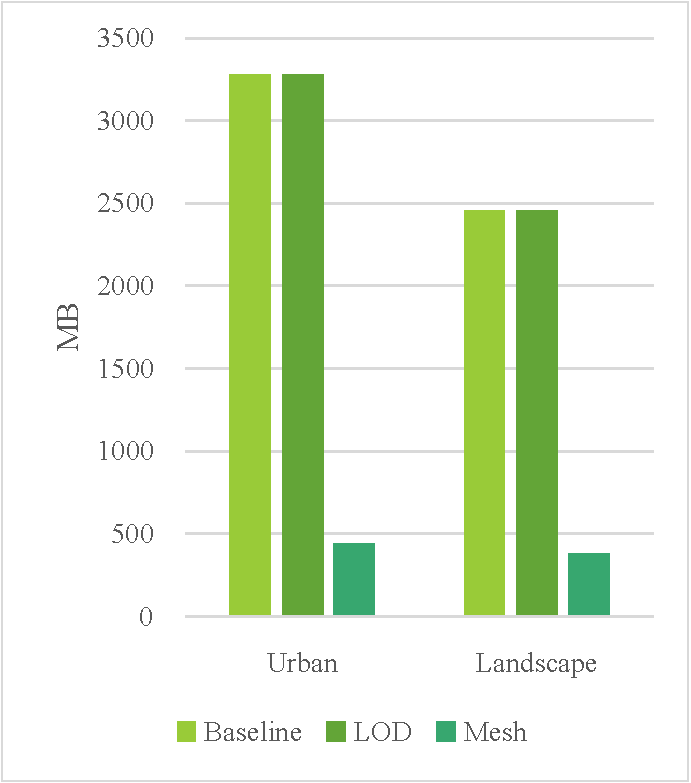
\includegraphics[width=\textwidth]{graph-mem-low.pdf}
        \caption{Low quality}
    \end{subfigure}
    
    \caption{Framerate measured on different quality settings.}
    \label{fig:results:graph-mem}
\end{figure}

The Mesh generation method uses 5.9x to 7.3x times less memory than baseline on urban scene and 5.4x to 6.4x times less memory on landscape scene.

Due to implementation peculiarities, the LOD generation algorithm uses the same amount of memory as the baseline.

\section{Limitations}

\subsection{LOD generation}

The LOD generation algorithm shows good visual quality when observing the scene from a far distance. However, due to the nature of point clouds, it loses detail in a close look. Furthermore, as there is a distance between points, the zoomed point cloud becomes hard to observe.

\begin{figure}[h]
    \centering
    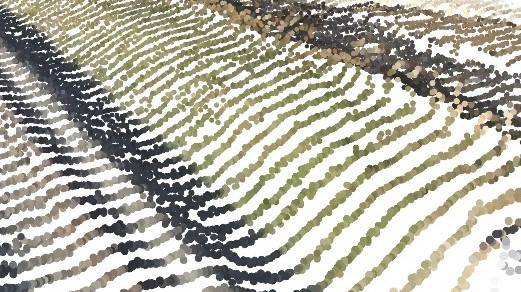
\includegraphics[width=0.7\textwidth]{lod-limitation.jpg}
    \caption{Point cloud visualised with LOD generation algorithm in close look.}
    \label{fig:results:lod-limitation}
\end{figure}

\subsection{Mesh generation}

Although the Mesh generation algorithm demonstrates excellent performance and detail, it has a fundamental flaw: this algorithm cannot correctly handle the scenes with objects placed above the ground, so there is a space between the surface and the object. Examples are bridges, trees, cranes, flying objects. This case is demonstrated on \autoref{fig:results:mesh-edgecase}.

As the algorithm records the highest point of the point cloud, the result will appear as a hill with all the details discarded under it.

\begin{figure}[h]
    \centering
    
    \begin{subfigure}{0.45\textwidth}
        \centering
        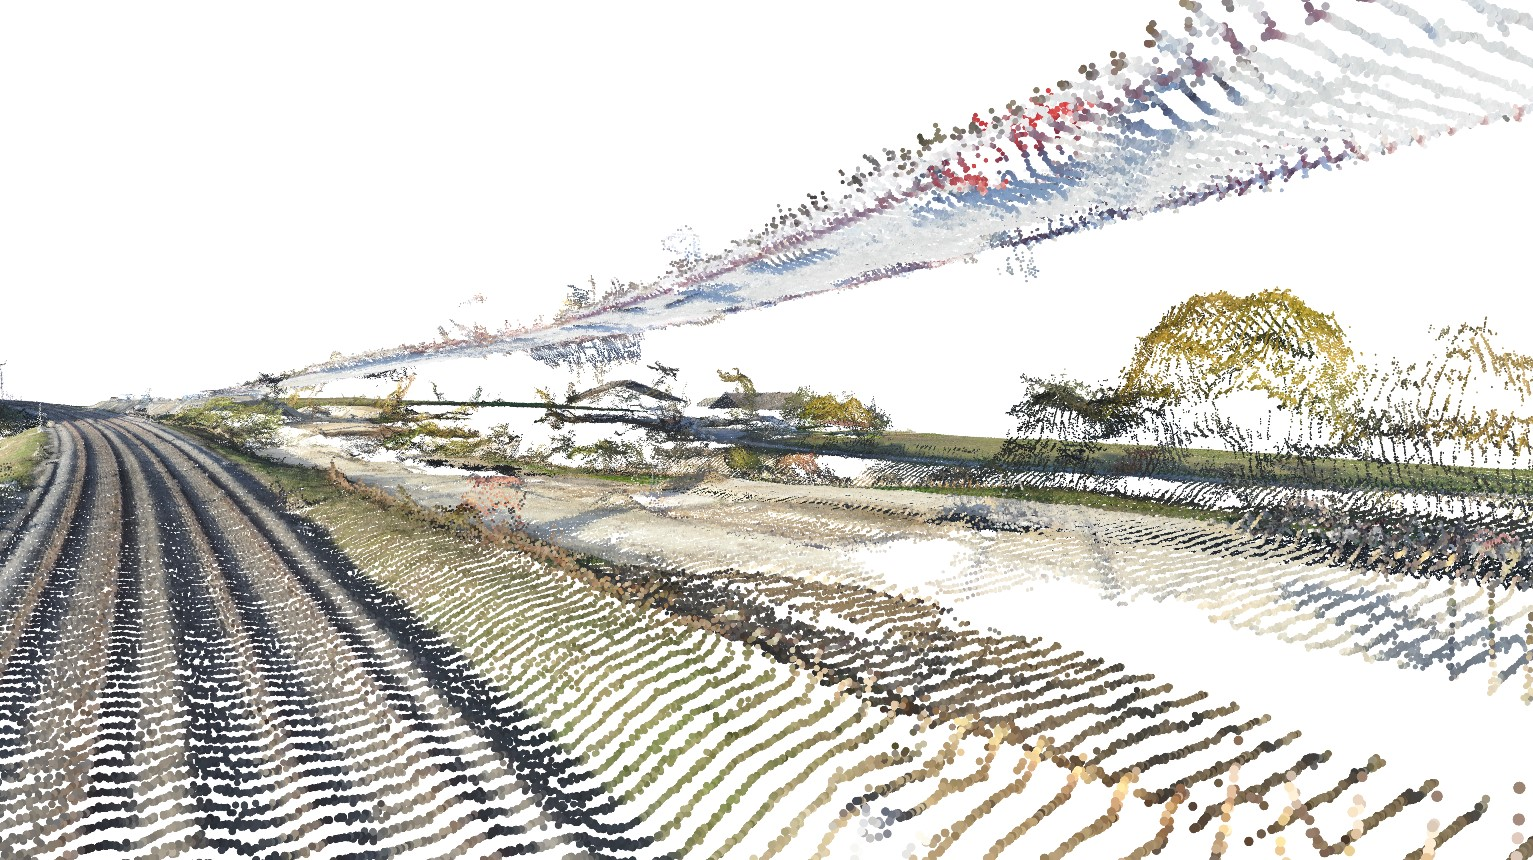
\includegraphics[width=\textwidth]{lod-edgecase.jpg}
        \caption{LOD generation. result}
    \end{subfigure}
    %
    \begin{subfigure}{0.45\textwidth}
        \centering
        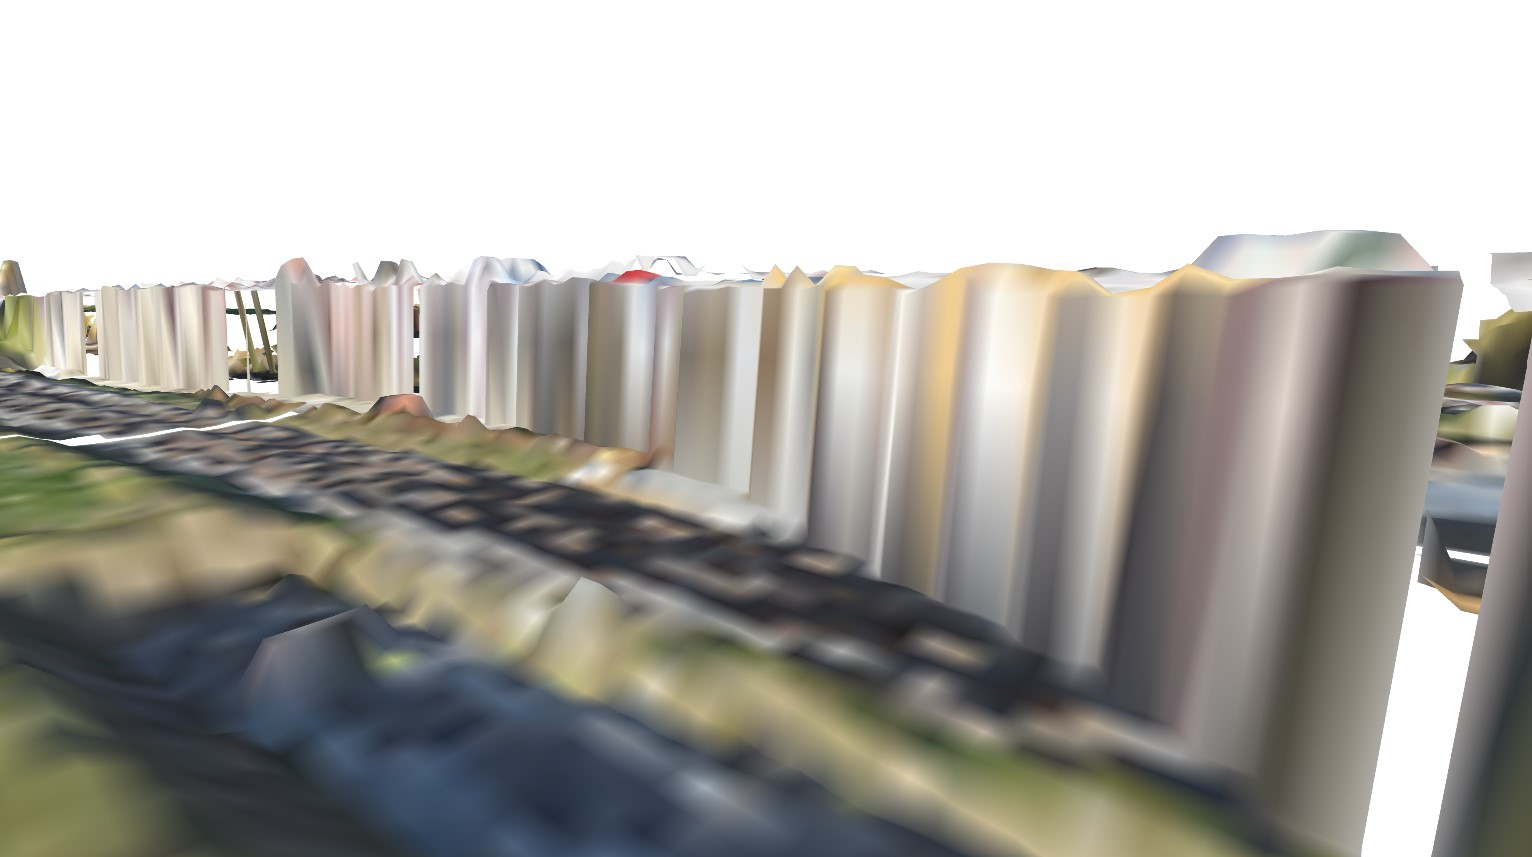
\includegraphics[width=\textwidth]{mesh-edgecase.jpg}
        \caption{Mesh creation result.}
    \end{subfigure}
    
    \caption{An example of edge case for mesh generation algorithm. It discards the detail under the bridge.}
    \label{fig:results:mesh-edgecase}
\end{figure}

Another problem is that the current implementation of the Mesh generation algorithm currently produces noticeable gaps on chunk borders. However, this defect can be eliminated in future work.

\subsection{Preprocessing}

The methods proposed in this work are designed for application before the run time. It means that one should execute them in advance. This limitation renders the methods inapplicable for real-time usage, except running in the background in a parallel process.

\subsection{Execution time}

Despite having a linear time complexity, the execution time might be more than a minute on large files (more than 1.5 GiB).

\section{Discussion}

It was observed that the Mesh generation method shows a higher performance boost when comparing to the LOD generation method. Mesh generation also uses significantly less memory than LOD generation. However, it has a significant drawback that was discussed above.

The LOD generation algorithm produces good results for observing point clouds from a far perspective. It keeps the detail of the point cloud and correctly handles the complex cases like floating objects that the Mesh generation algorithm might handle erratically. However, it is not applicable for close or precise object examination.

The Mesh generation algorithm should be applicable in most cases. For example, it produces good results when visualizing open landscape areas with simple geometry. Therefore, the Innopolis Simulator team decided to use the Mesh generation in the simulator software.

One might use the LOD generation algorithm for examining the raw point clouds as it visualizes the cloud in its unprocessed form with better performance.

A user should explore the algorithm capabilities and limitations and input data features and choose a suitable algorithm based on these observations.



%% REFERENCES
\printbibliography[heading=bibintoc,title={Bibliography cited}]

%% APPENDIX
\appendix

\chapter{Rendered scenes}
\label{appex:rendered-scenes}

\begin{figure}[h]
    \centering
    
    \begin{subfigure}{0.9\textwidth}
        \centering
        \includegraphics[width=\textwidth]{figs/results/lod-urban-800.jpg}
        \caption{LOD 800-1600-3200}
    \end{subfigure}
    
    \begin{subfigure}{0.9\textwidth}
        \centering
        \includegraphics[width=\textwidth]{figs/results/lod-urban-400.jpg}
        \caption{LOD 400-800-1600}
    \end{subfigure}
    
    \begin{subfigure}{0.9\textwidth}
        \centering
        \includegraphics[width=\textwidth]{figs/results/lod-urban-200.jpg}
        \caption{LOD 200-800-1600}
    \end{subfigure}
    
    \caption{Urban scene rendered with LODs.}
\end{figure}

\begin{figure}[h]
    \centering
    
    \begin{subfigure}{0.7\textwidth}
        \centering
        \includegraphics[width=\textwidth]{figs/results/lod-landscape-300.jpg}
        \caption{LOD 300-600-1200}
    \end{subfigure}
    
    \begin{subfigure}{0.7\textwidth}
        \centering
        \includegraphics[width=\textwidth]{figs/results/lod-landscape-200.jpg}
        \caption{LOD 200-400-800}
    \end{subfigure}
    
    \begin{subfigure}{0.7\textwidth}
        \centering
        \includegraphics[width=\textwidth]{figs/results/lod-landscape-100.jpg}
        \caption{LOD 100-200-400}
    \end{subfigure}
    
    \caption{Landscape scene rendered with LODs.}
\end{figure}

\begin{figure}[h]
    \centering
    
    \begin{subfigure}{0.9\textwidth}
        \centering
        \includegraphics[width=\textwidth]{figs/results/mesh-urban-256.jpg}
        \caption{Mesh w. chunk resolution 256}
    \end{subfigure}
    
    \begin{subfigure}{0.9\textwidth}
        \centering
        \includegraphics[width=\textwidth]{figs/results/mesh-urban-128.jpg}
        \caption{Mesh w. chunk resolution 128}
    \end{subfigure}
    
    \begin{subfigure}{0.9\textwidth}
        \centering
        \includegraphics[width=\textwidth]{figs/results/mesh-urban-64.jpg}
        \caption{Mesh w. chunk resolution 64}
    \end{subfigure}
    
    \caption{Urban scene rendered with generated mesh.}
\end{figure}

\begin{figure}[h]
    \centering
    
    \begin{subfigure}{0.7\textwidth}
        \centering
        \includegraphics[width=\textwidth]{figs/results/mesh-landscape-256.jpg}
        \caption{Mesh w. chunk resolution 256}
    \end{subfigure}
    
    \begin{subfigure}{0.7\textwidth}
        \centering
        \includegraphics[width=\textwidth]{figs/results/mesh-landscape-128.jpg}
        \caption{Mesh w. chunk resolution 128}
    \end{subfigure}
    
    \begin{subfigure}{0.7\textwidth}
        \centering
        \includegraphics[width=\textwidth]{figs/results/mesh-landscape-64.jpg}
        \caption{Mesh w. chunk resolution 64}
    \end{subfigure}
    
    \caption{Landscape scene rendered with generated mesh.}
\end{figure}


\end{document}
